\chapter{Simulations} \label{chap-3}

Holmes et al. recently performed PIC simulations in the original ORBIT code to determine the feasibility of elliptical painting in the SNS \cite{Holmes2018}. Their findings are reviewed in this chapter. Additionally, the simulations are extended in PyORBIT to include updated experimental constraints. First, the computational model is briefly described. 


\section{Computational model}

The PyORBIT code tracks a Bunch object containing the 6D phase space coordinates. The accelerator is modeled as a series of nodes, each of which modifies the phase space coordinates in some way. Following the TEAPOT approach [\ref{}], single particles are transported using symplectic maps derived from the Hamiltonian. Here, we briefly describe the approach to nonlinear magnetic fringe fields and collective effects. 


\subsection{Space charge}

A major component of beam physics simulations is the calculation of the space charge force. Direct Coloumb sums are currently infeasible. The Vlasov equation can be solved directly, but this is difficult in 2D and 3D. The particle-in-cell (PIC) method is a “best of both worlds” approach in which an $N$ particle bunch is represented by $M$ macroparticles, where $M \ll N$. The macroparticles are tracked according to Eq.~\eqref{eq:eom_with_spacecharge}. The electric field is obtained by solving Eq.~\eqref{eq:Poisson} on a grid. The key step is transforming between the discrete and continuous representation. The PIC loop is shown in Fig.~\ref{fig:pic_loop}. 
%
\begin{figure}[!p]
    \centering
    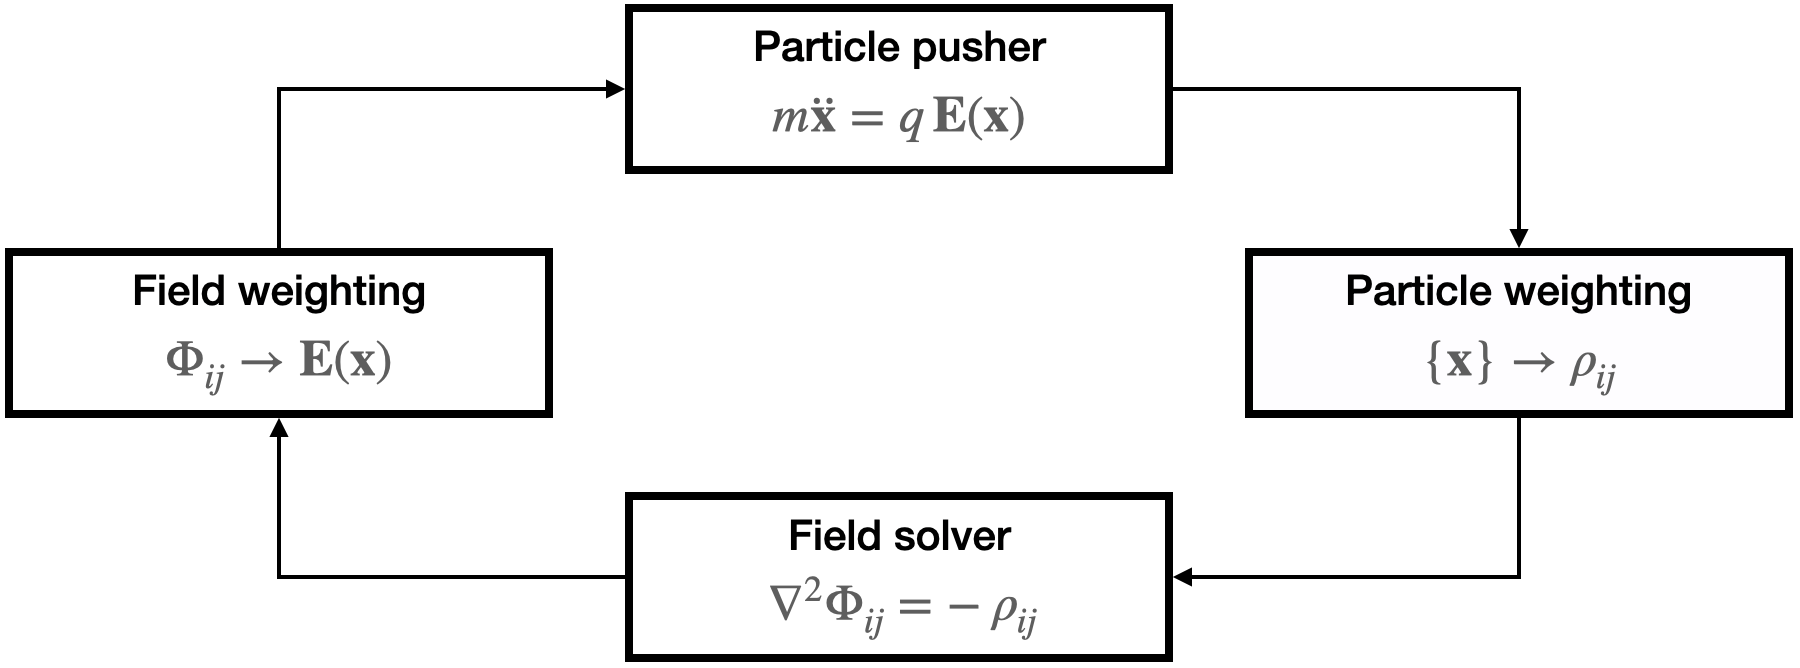
\includegraphics[width=\textwidth]{Images/chapter3/pic_loop.png}
    \caption{\label{fig:pic_loop}The particle-in-cell loop.}
    \vfill
    \vspace*{2.5cm}
    \vfill
    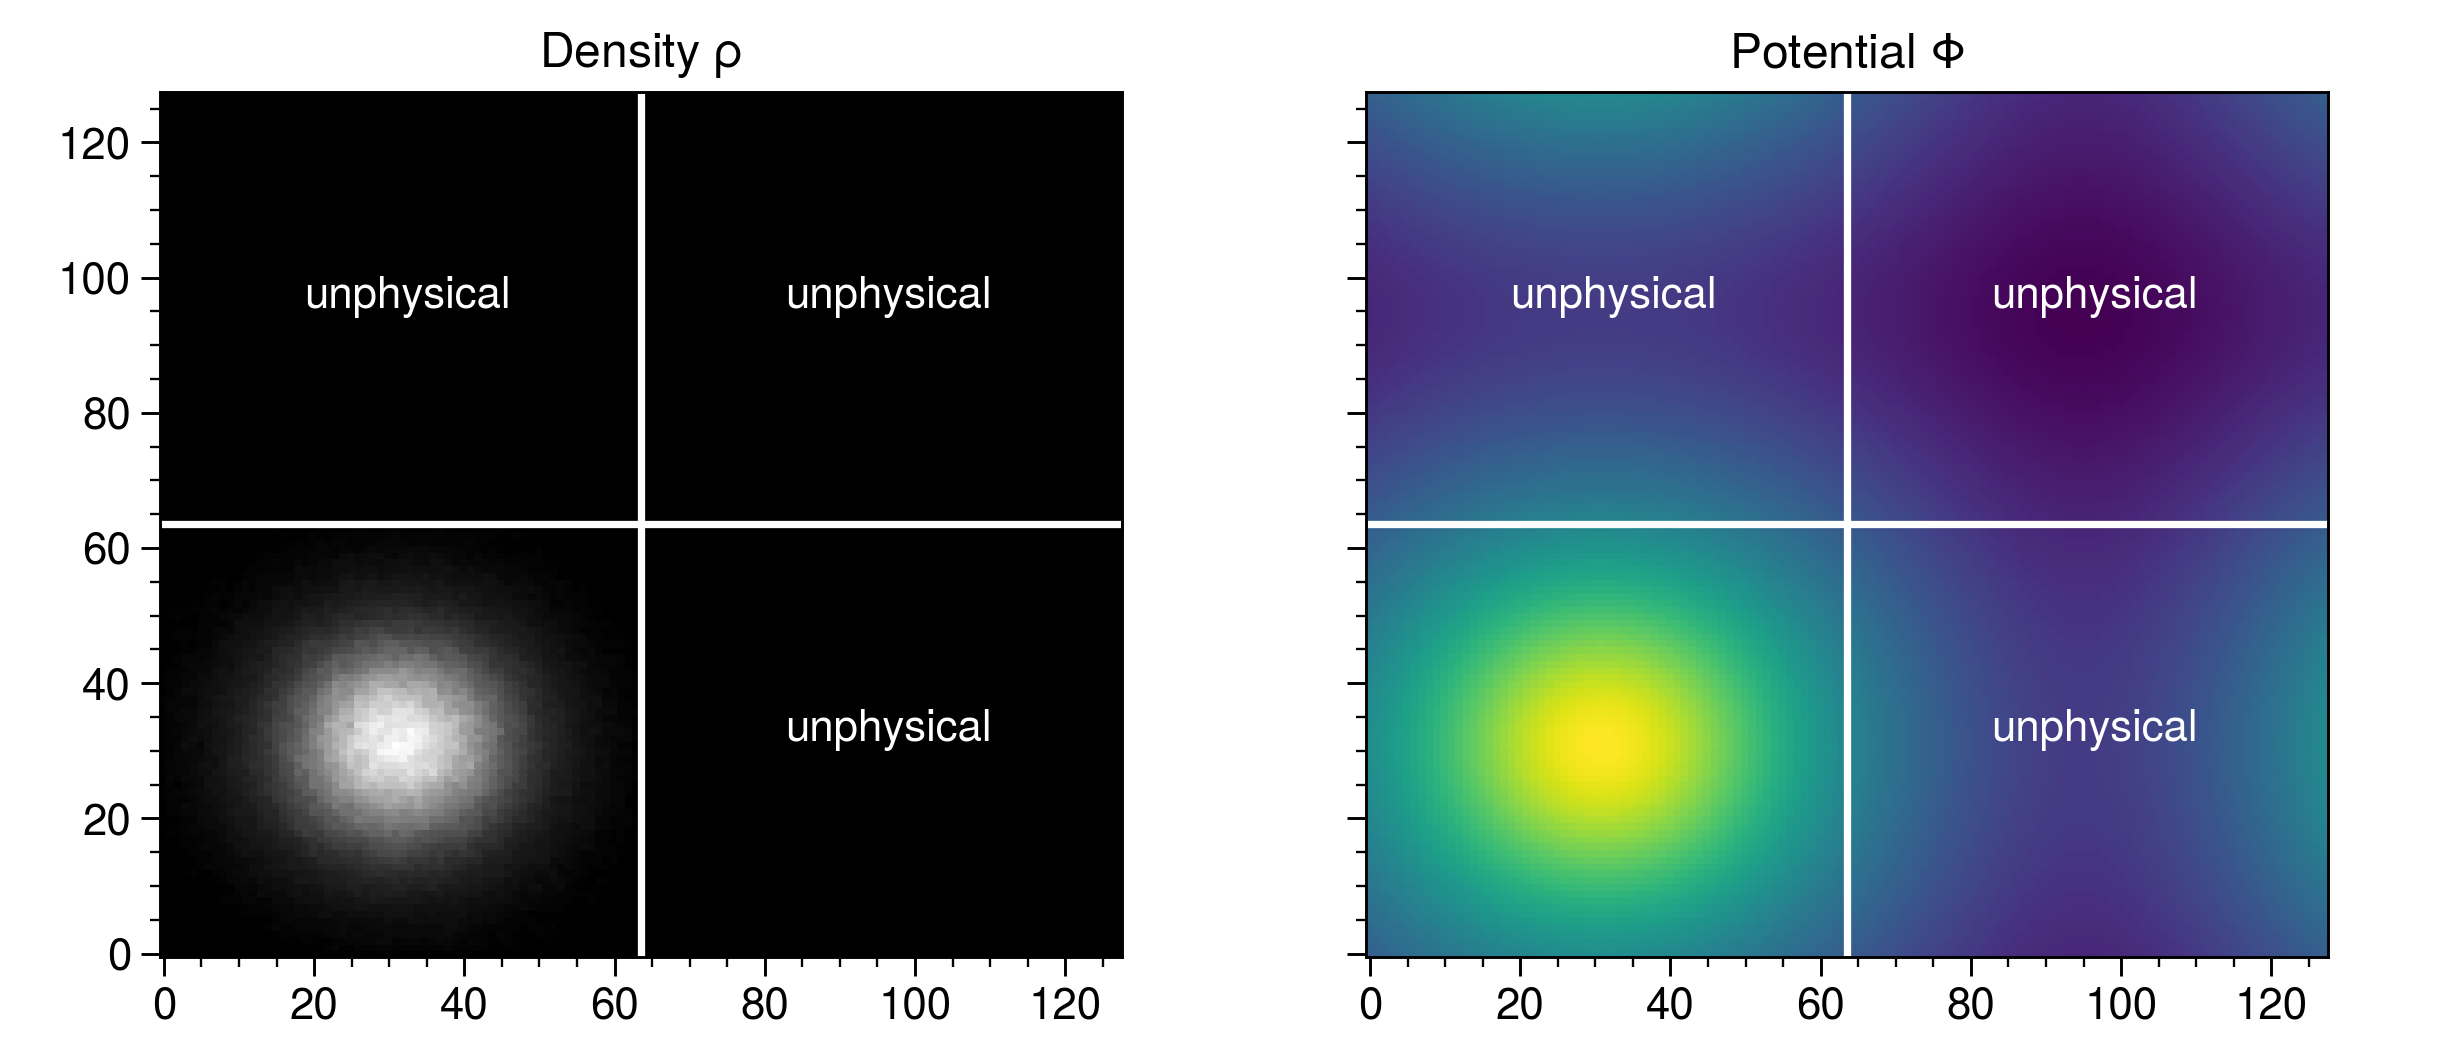
\includegraphics[width=\textwidth]{Images/chapter3/poisson.png}
    \caption{\label{fig:poisson}Solution of Poisson's equation on a doubled grid.}
    
\end{figure}
%

First, the charge density $\rho_{i,j}$ is obtained on a grid. A common method is to treat each macroparticle as a rectangular, uniform density cloud of charge with dimensions equal to the grid spacing, assigning a fractional charge to each bin according to the fraction of the cloud overlapping with that bin \cite{Birdsall1975}. Second, Poisson’s equation is solved on the grid. The method used in PyORBIT follows \cite{Hockney1981}. The potential is written as the convolution of a Green's function $G(\mathbf{x})$ with the charge density $\rho(\mathbf{x})$:
%
\begin{equation}
    \Phi(\mathbf{x}) = G(\mathbf{x}) * \rho(\mathbf{x}).
\end{equation}
%
We then exploit the convolution theorem \cite{Arfken1985} to write
%
\begin{equation}
    \mathcal{F}[\Phi(\mathbf{x})]
    =
    \mathcal{F}[G(\mathbf{x})] \cdot \mathcal{F}[\rho(\mathbf{x})]
\end{equation}
%
where $\mathcal{F}$ represents the Fourier transform. For a grid with $N$ bins per dimension, the time-complexity of the convolution is $O(N^2)$. The Fourier transform reduces this to $O(N \log N)$. To create periodic boundary conditions, the grid is doubled in each dimension. The Green's function is mirror-reflected onto these new regions, while the charge density is set to zero. The potential is solved for on the extended grid, after which the unphysical regions are discarded. An example is shown in Fig.~\ref{fig:poisson}. Third, using the same weighting method as the first step, the gradient of the potential is interpolated at the particle positions. Finally, the particle momenta are updated using an appropriate integration scheme.

Care must be taken when choosing the number of macroparticles, grid size, and integration step size. In the following simulations, 128 bins are used in each dimension. The number of macroparticles changes during injection, but the final number of particles is usually at least $3 \times 10^{5}$.

In rings where the coasting beam approximation is valid, the longitudinal and transverse dimensions are treated separately. In PyORBIT, a longitudinal space charge node acts on the bunch once per turn. Two models are included for the transverse space charge calculation: the 2.5D model and the sliced model. In the 2.5D model, Poisson’s equation is solved once for a charge density obtained by projecting the entire bunch onto the $x$-$y$ plane; the transverse space charge forces are then weighted according to the longitudinal density. In the sliced model, the bunch is longitudinally sliced, and Poisson’s equation is solved for each slice. 

\subsection{Wake fields, fringe fields, and other effects}

In the discussion of space charge thus far, the beam was assumed to be in free space. In reality, the beam is in a conducting vacuum chamber. Charged particles leave so-called wake fields on the conducting surface, which then act on other particles or on the same particle in a ring, possibly leading to instability. The treatment of wake fields can be challenging and is introduced in \cite{Chao1993}. No details are described here; we just mention that PyORBIT takes these effects into account.

Quadrupole, dipole, and solenoid magnets are finite in length; the magnetic fields outside the core are nonlinear. These are referred to as fringe fields. [...]

An important effect during charge-exchange injection is Coulomb scattering during passage through the stripper foil. [...].

Finally, longitudinal focusing in the ring is provided by two RF cavities. The harmonic frequency $h$ is defined as the RF frequency divided by the revolution frequency of the beam; one cavity operates at $h = 1$ and the other operates at $h = 2$, both at an amplitude near 5 kV. The energy gain $\Delta \epsilon$ for a particle passing through the cavity is approximated as  
%
\begin{equation}
    \Delta \epsilon = q V \sin(h \phi + \phi_0).
\end{equation}
%
The particle phase $\phi$ is zero for the synchronous particle.



\section{Fringe field compensation}

It was found in \cite{Holmes2018} that in an otherwise linear lattice, fringe fields tend to eliminate any cross-plane correlations in the beam when the tunes are near the difference resonance $\nu_x \approx \nu_y$. To demonstrate this, we generate a Danilov distribution matched to a linearized version of the SNS ring. Fringe fields are then turned on, and the particles are tracked without space charge. Fig.~\ref{fig:fringe_a} shows the turn-by-turn evolution.
%
\begin{figure}[!p]
    \centering
    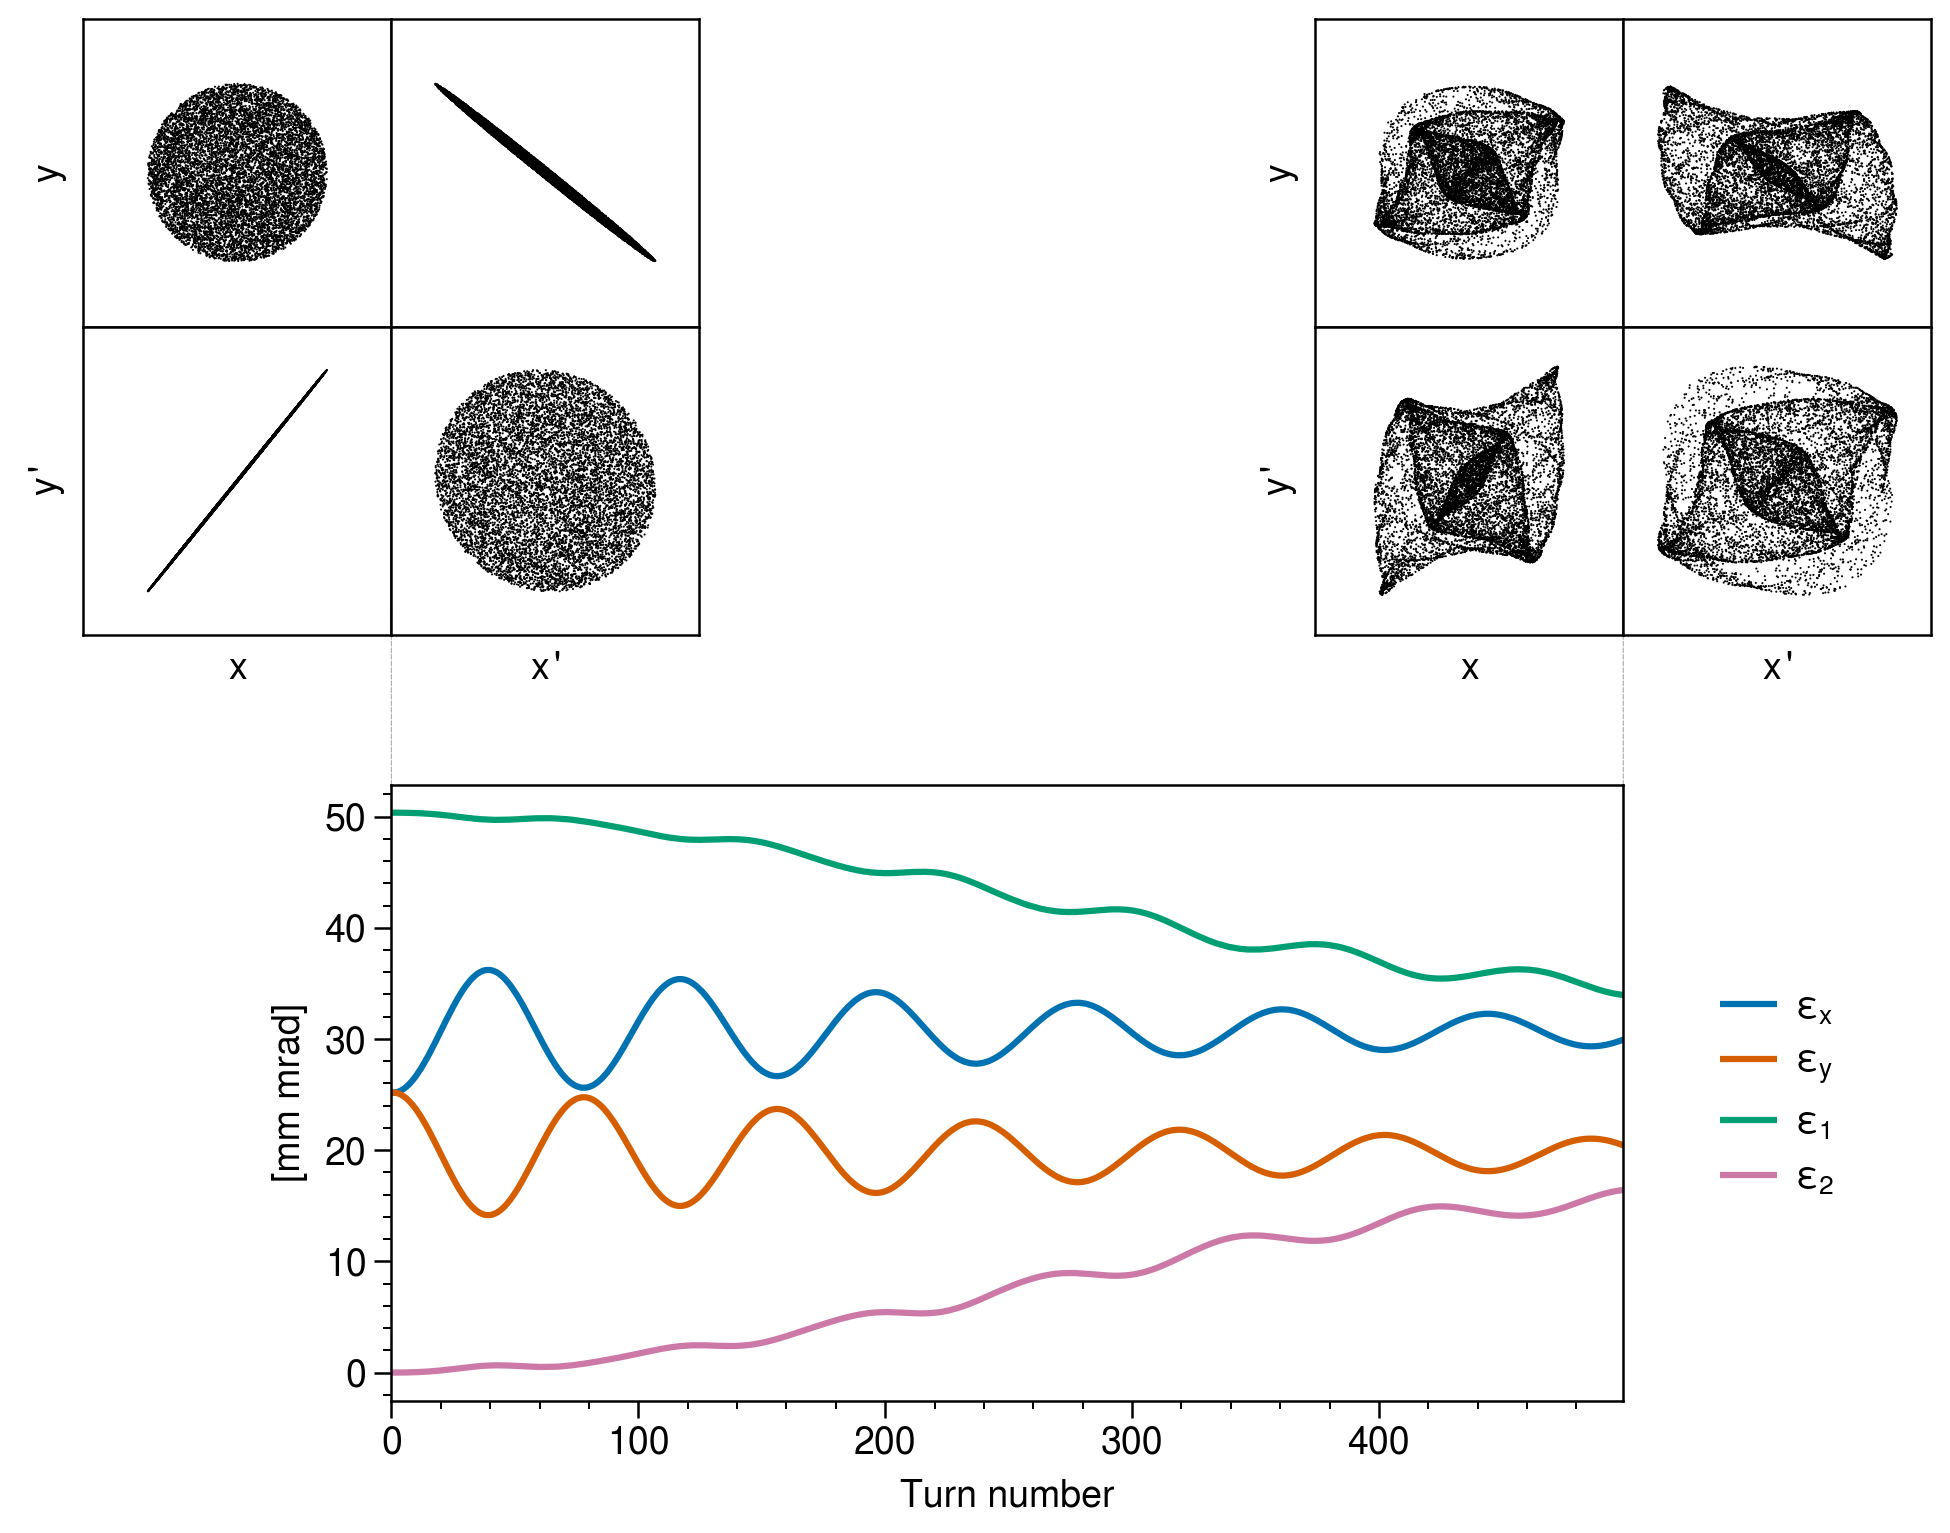
\includegraphics[width=0.7\textwidth]{Images/chapter3/fringe.png}
    \caption{Danilov distribution tracked in the SNS ring. Fringe fields are the only nonlinear external effect.}
    \label{fig:fringe_a}
    \vspace*{3cm}
\end{figure}
%
%
\begin{figure}[!p]
    \centering
    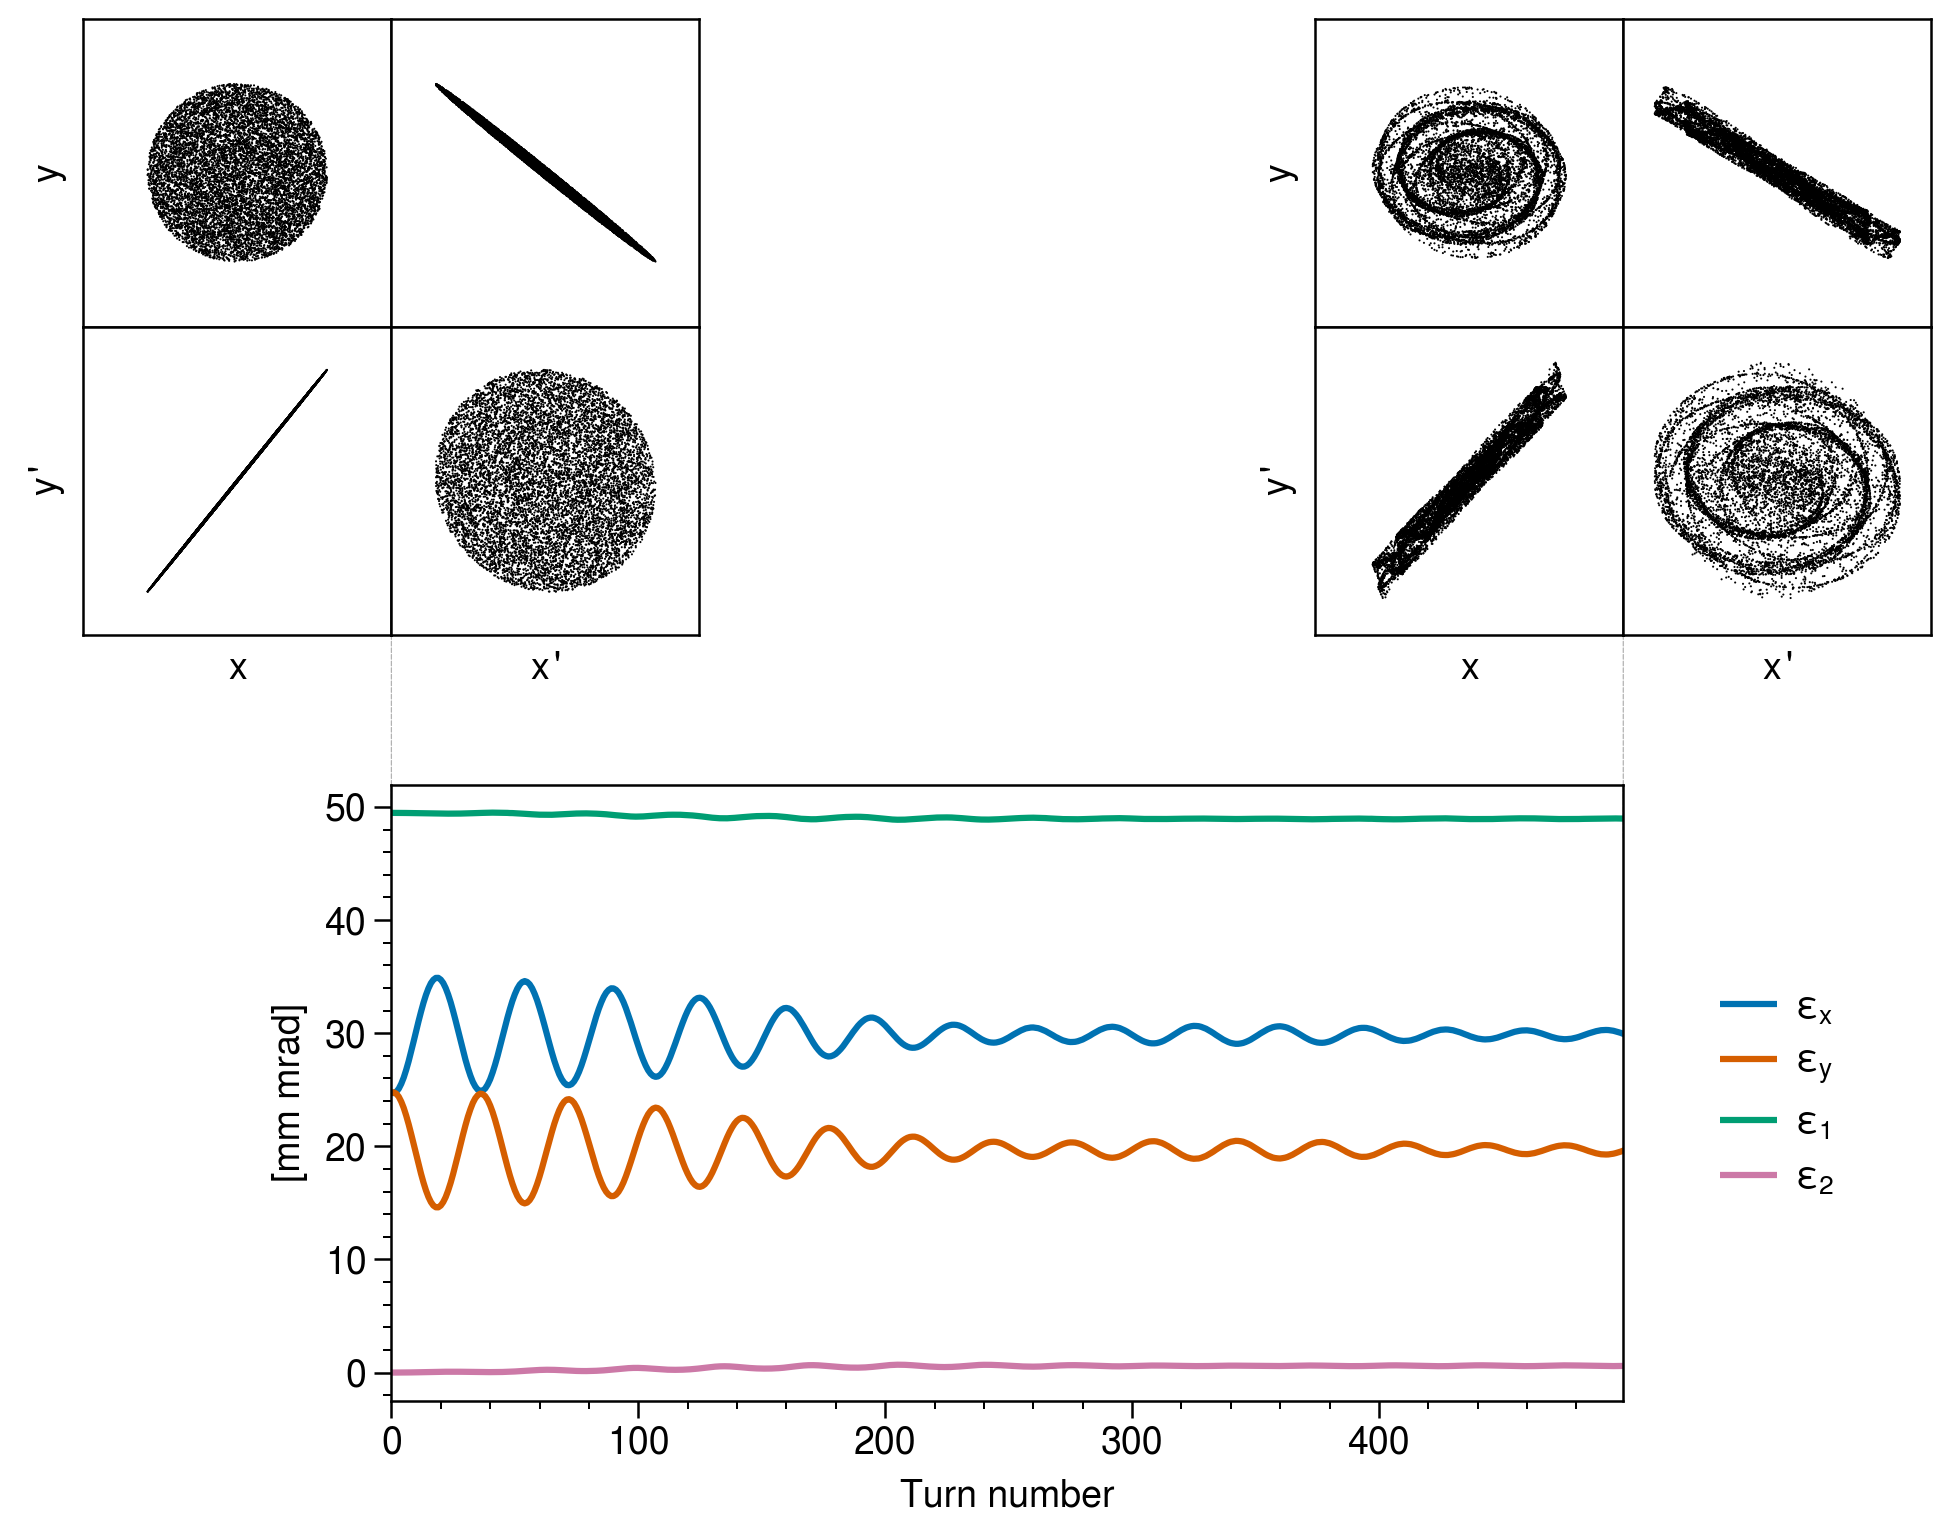
\includegraphics[width=0.7\textwidth]{Images/chapter3/fringe_solenoid.png}
    \caption{Danilov distribution tracked in the SNS ring with a solenoid added to the ring. Fringe fields are the only nonlinear external effect.}
    \label{fig:fringe_b}
    \vspace*{3cm}
\end{figure}
%
%
\begin{figure}[!p]
    \centering
    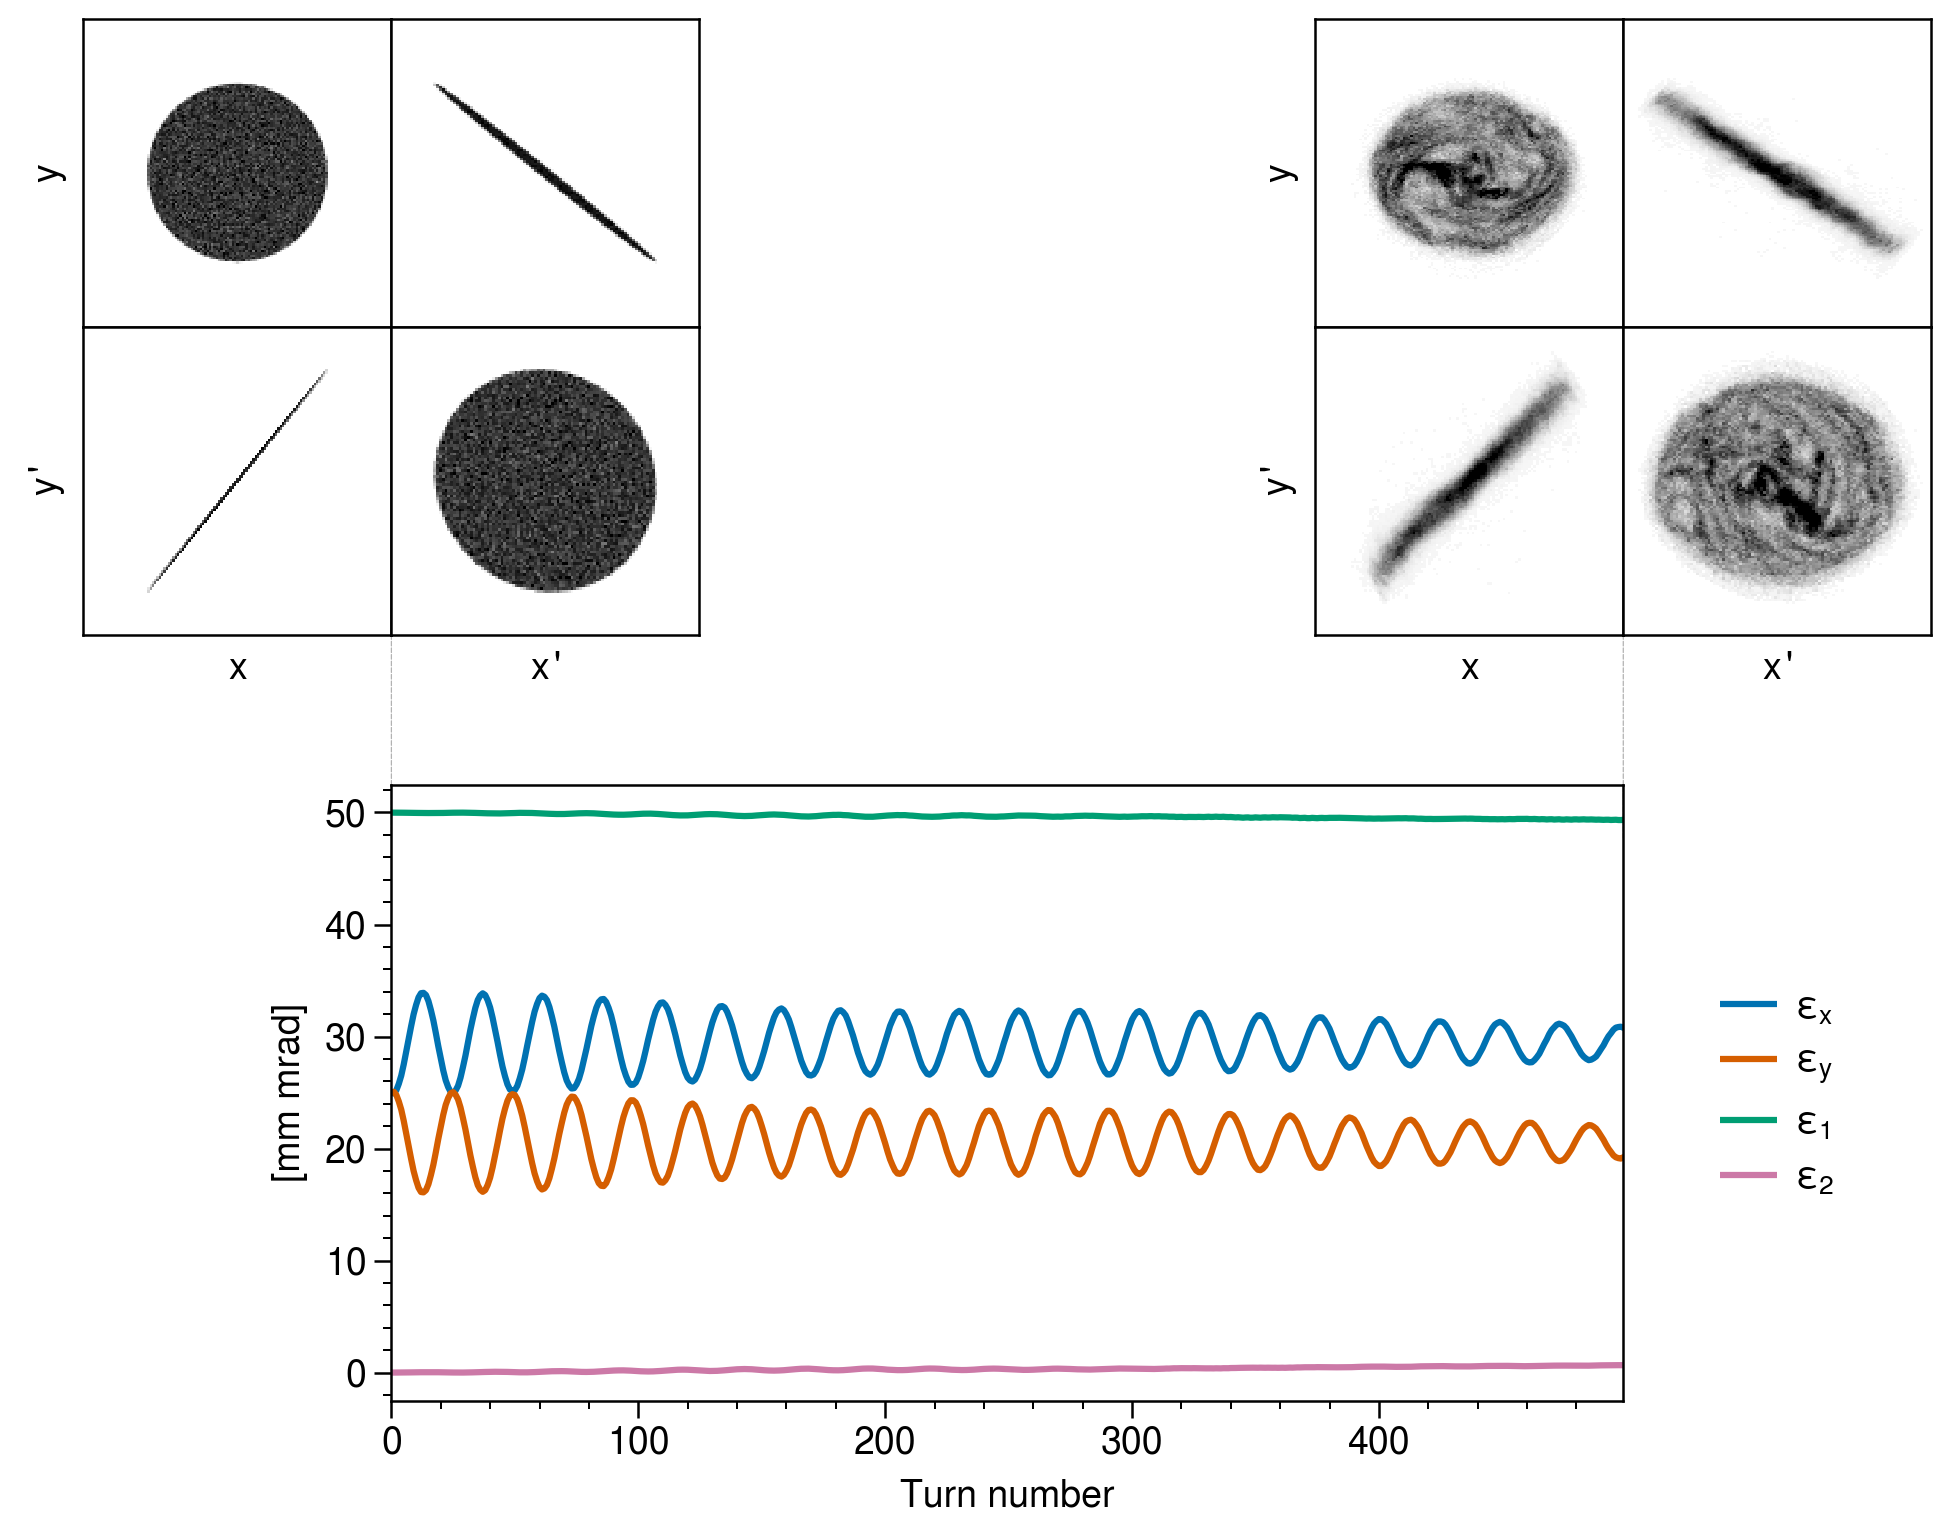
\includegraphics[width=0.7\textwidth]{Images/chapter3/fringe_spacecharge.png}
    \caption{Danilov distribution tracked in the SNS ring with space charge. Fringe fields are the only nonlinear external effect.}
    \label{fig:fringe_c}
    \vspace*{3cm}
\end{figure}
%

There is clearly nonlinear coupling between the horizontal and vertical motion; the final distribution is a superposition of rotating and counter-rotating modes. In ...

Although the effect of fringe fields is still noticeable, the cross-plane correlations are mostly maintained. The tunes $\nu_{1, 2}$ are no longer equal due to the linear coupling form the solenoid, so the resonance condition is avoided. In Fig.~\ref{fig:fringe_c}, the simulation is repeated with the inclusion of space charge instead of the solenoid magnet. An intensity of $10^{14}$ is used and the bunch length is equal to the ring length. We see that space charge has a similar stabilizing effect on the distribution.


\section{Painting simulations}

The injection process is simulated by adding particles to the bunch at the foil location on each turn. The minipulse from the linac has an RMS emittance of approximately 0.3 mm~mrad. A so-called JOHO distribution is used:
%
%
The beam Twiss parameters are usually assumed to be matched to the lattice ($\beta_x \approx \beta_y \approx 10$ m/rad, $\alpha_x \approx \alpha_y \approx 0$ rad), but recent measurements indicate that they could be significantly different, particularly the $\alpha$ parameter which determines the beam divergence. To be safe, we use values close to these measurements. A Gaussian distribution is used for the longitudinal distribution with RMS energy spread of a few MeV. Since the minipulse is much smaller than the final accumulated pulse, the exact details of the minipulse distribution are not important.


\begin{figure}[!p]
    \centering
    \begin{subfigure}{\textwidth}
        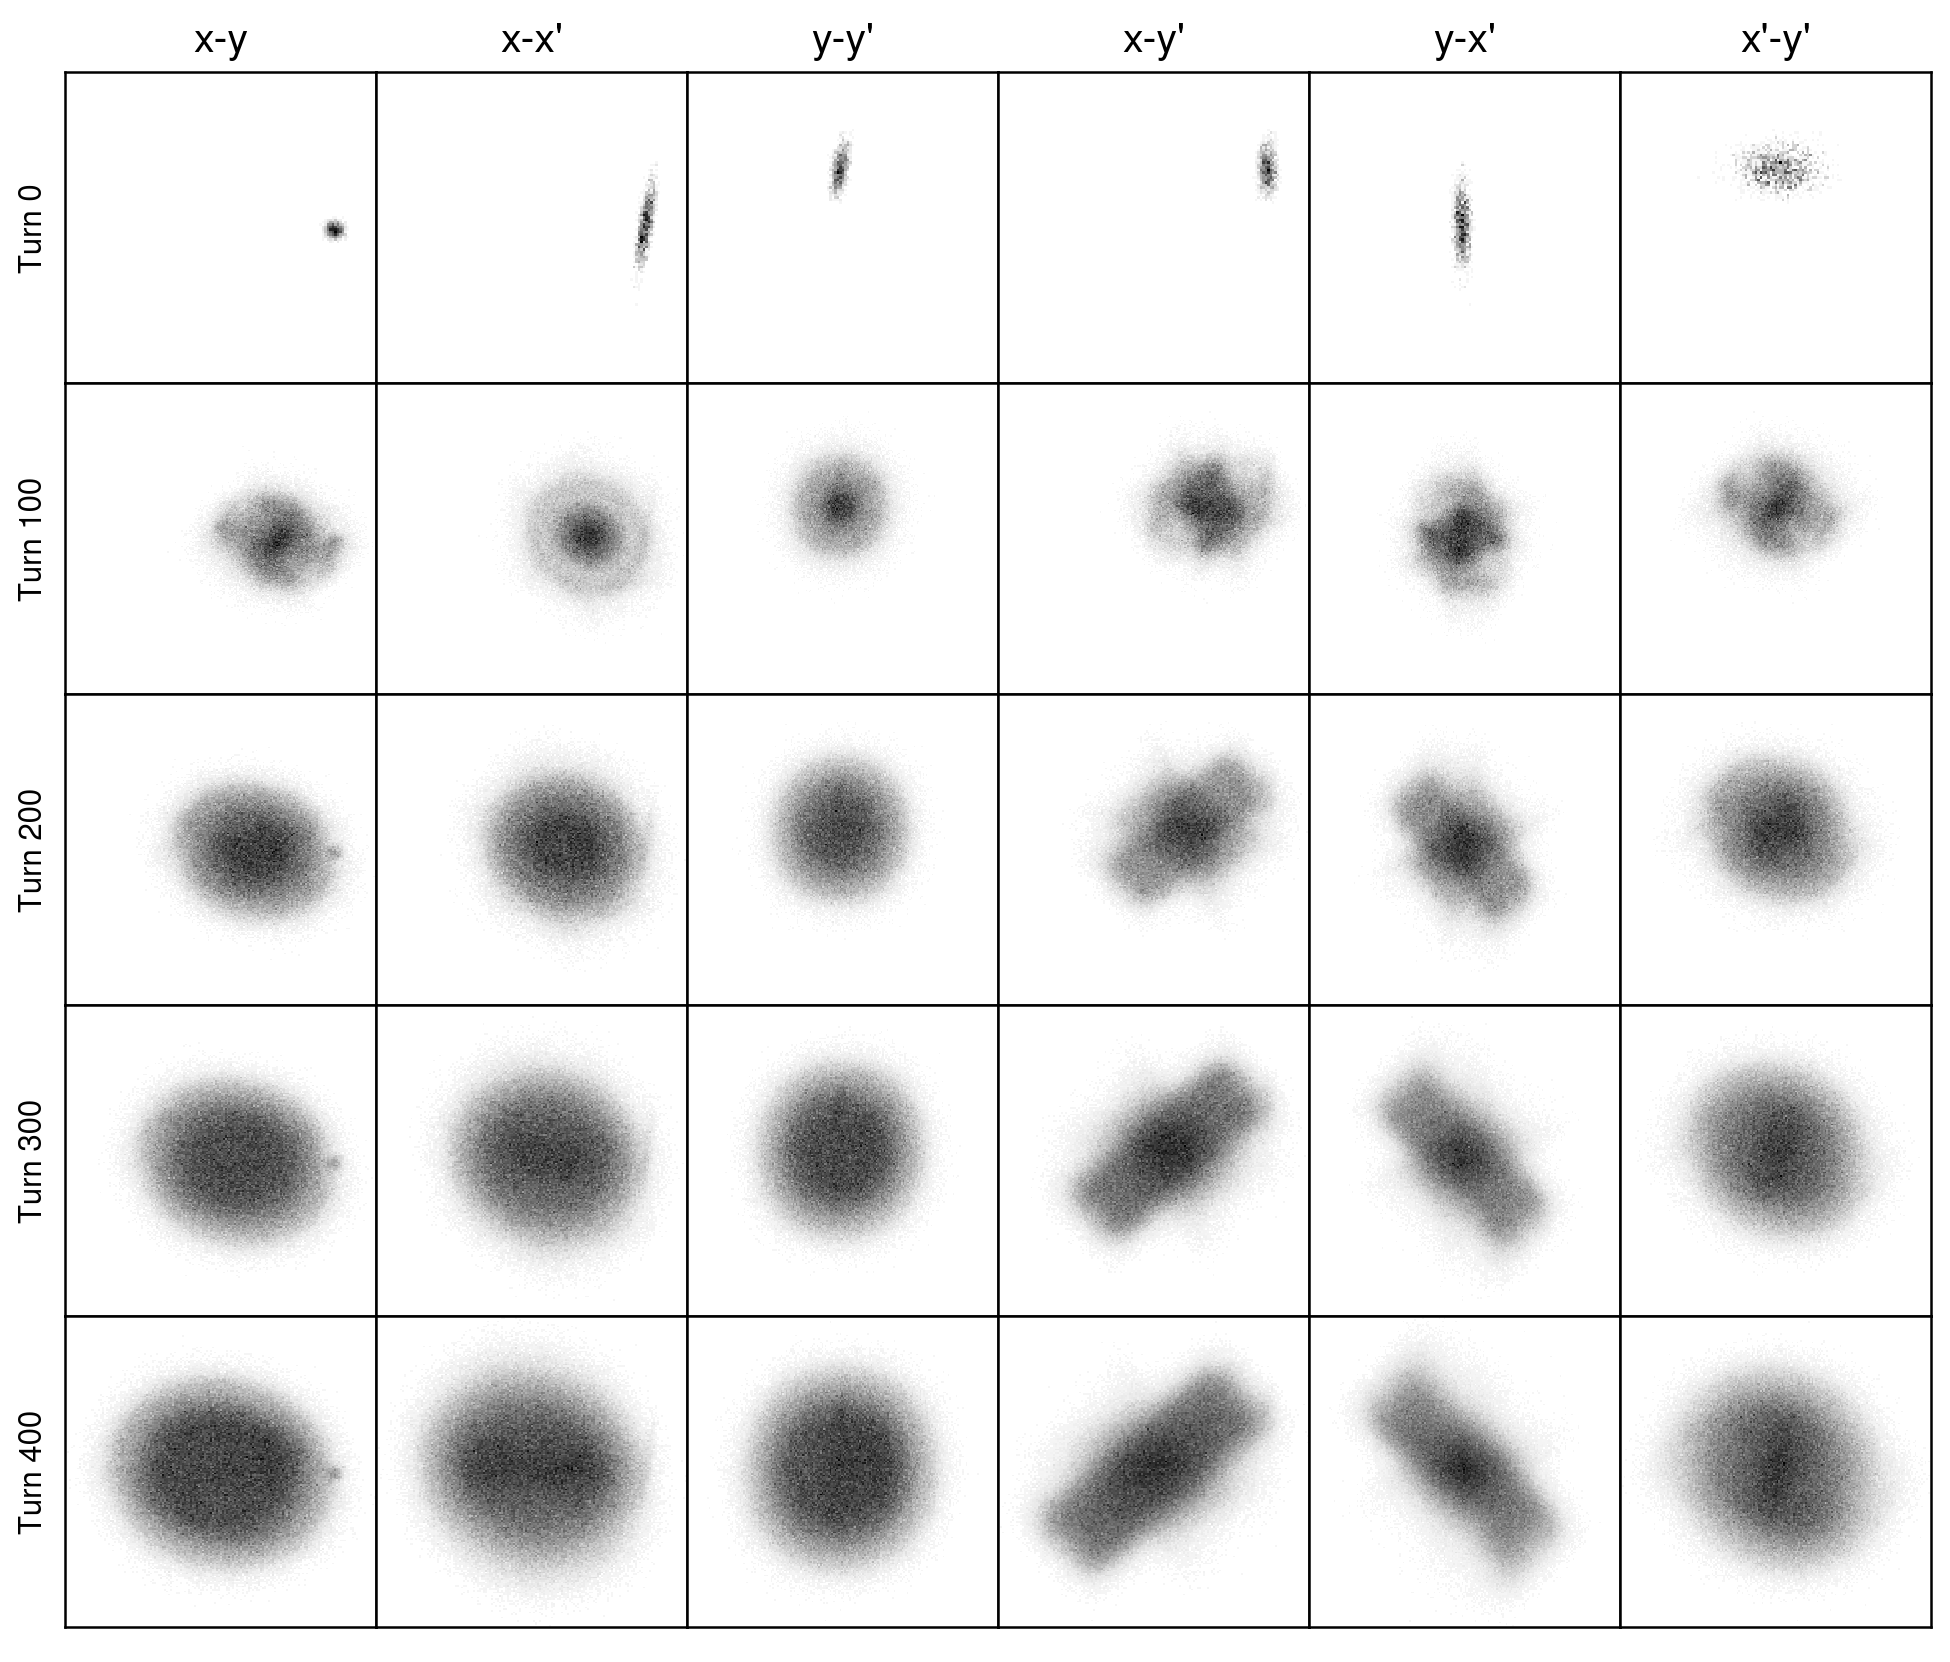
\includegraphics[width=\textwidth]{Images/chapter3/snapshots.png}
    \end{subfigure}
    \vfill
    \vspace*{1.0cm}
    \vfill
    \begin{subfigure}{0.7\textwidth}
        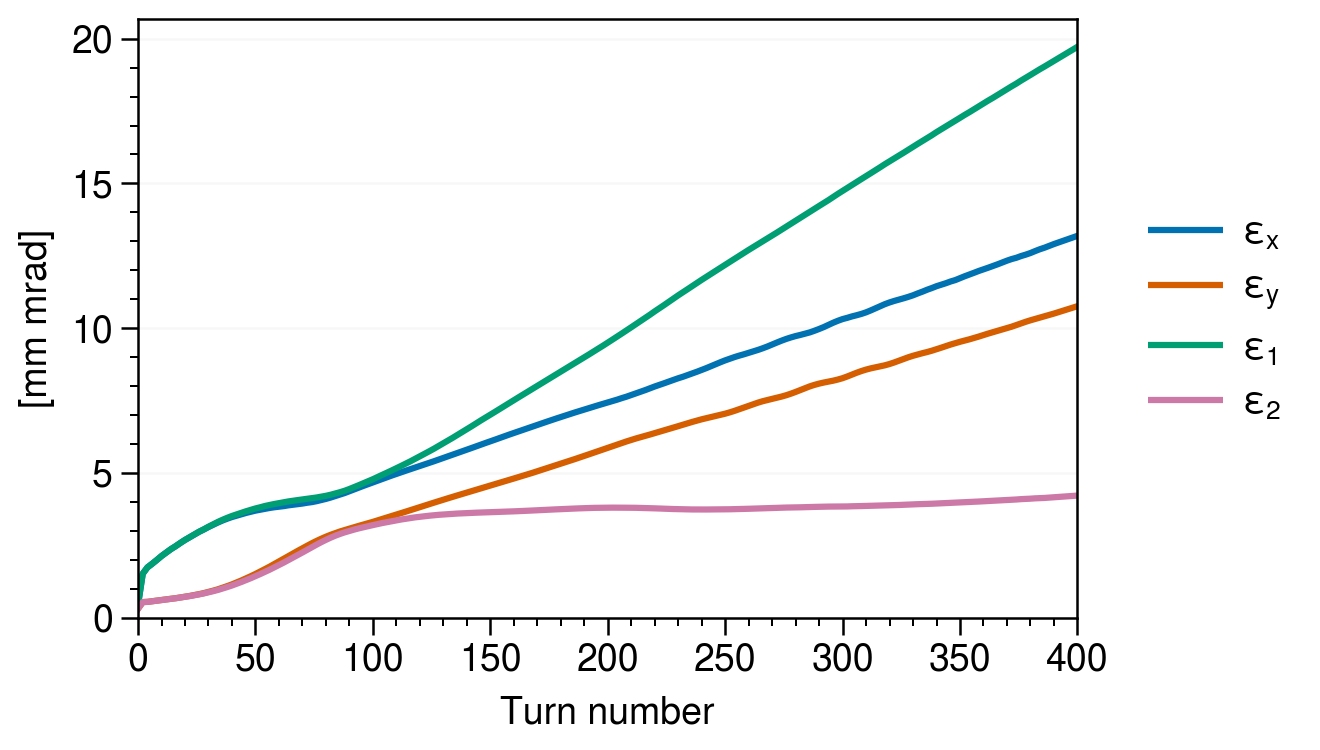
\includegraphics[width=\textwidth]{Images/chapter3/emittances.png}
    \end{subfigure}
    \caption{Simulation of elliptical painting.}
    \label{fig:my_label}
\end{figure}